\documentclass[Rapport/Rapport_main.tex]{subfiles}
\begin{document}
\subsection{WPF applikation}
Applikation er baseret på design mønsteret Model-View-ViewModel, som er et ofte anvendt mønster inden for WPF. Fordelene og ulemperne ved brug af MVVM er allerede beskrevet i de forrige afsnit, og ved ikke uddybes yderligere. Der er valgt en ViewFirst tilgang til designet, hvor Viewet laves først og derudfra laves præsentationslogikken i ViewModel. I de følgende afsnit beskrives mønsterets anvendelse i applikation, samt de generelle design overvejelser for Views og ViewModels. 

\subsubsection{Page Navigation}
En afgørende faktor for systemet er at kunne navigere mellem Views og ViewModels runtime. Et andet er at samtidigt opretteholde lav kobling og ingen direkte relation mellem View og ViewModel. Hvis hvert ViewModel selv havde til ansvar for at skifte mellem View, skulle de har direkte adgang til hvert ViewModel, samt hvert ViewModel skulle kende til tilhørende View, da de selv skulle stå for at initiere det. Dette strider både imod MVVM-arkitekturen, og skaber også høj kobling mellem ViewModellerne. Derfor udliciteres dette ansvar til klassen ApplicationViewModel. 

ApplicationViewModel består af en Usermodel (instans af den bruger som er logget ind), og en CurrentPage property, som er den side som vises på den grafiske brugeroverflade. Alle Views i systemet er prædefineret i ApplicationPage enumerationen, som anvendes til at konvertere til de konkrete view-instanser i ApplicationPageValueConverterklassen. Figur \ref{fig:PageNavigation_CD} viser et klassediagram for navigationsdesignet. ApplicationViewModellen er statisk og laves som en singleton, da alle sideskift er afhængige af hinanden (Man kan ikke vise to sider af gangen). 
\begin{figure}[H]
    \centering
    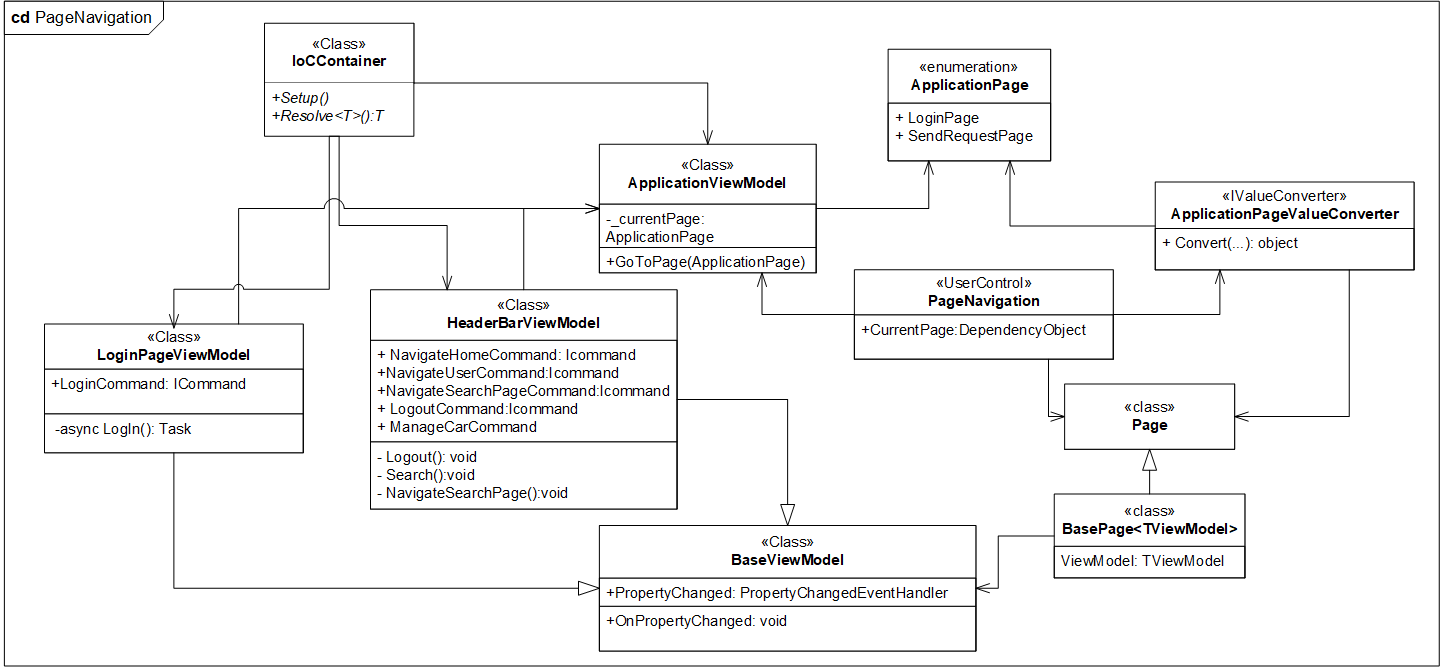
\includegraphics[width=\textwidth]{SoftwareDesign/MVVMDesigns/Graphics/PageNavigationcd.png}
    \caption{Her ses klassediagram for PageNavigation, hvor man ser de forskellige klasser involveret, når en side skal skiftes ud med en anden. Kun 2 ViewModels er inkluderet i diagrammet, men alle ViewModels har adgang til den statiske instans af ApplicationViewModel}
    \label{fig:PageNavigation_CD}
\end{figure}
Nedenfor ses et sekvensdiagram, som beskriver skiftet fra LoginView til StartPage. Her anvendes ViewModellens singleton instans af ApplicationViewModel til at skifte side med 'GoToPage'-metoden. 
\begin{figure}[H]
    \centering
    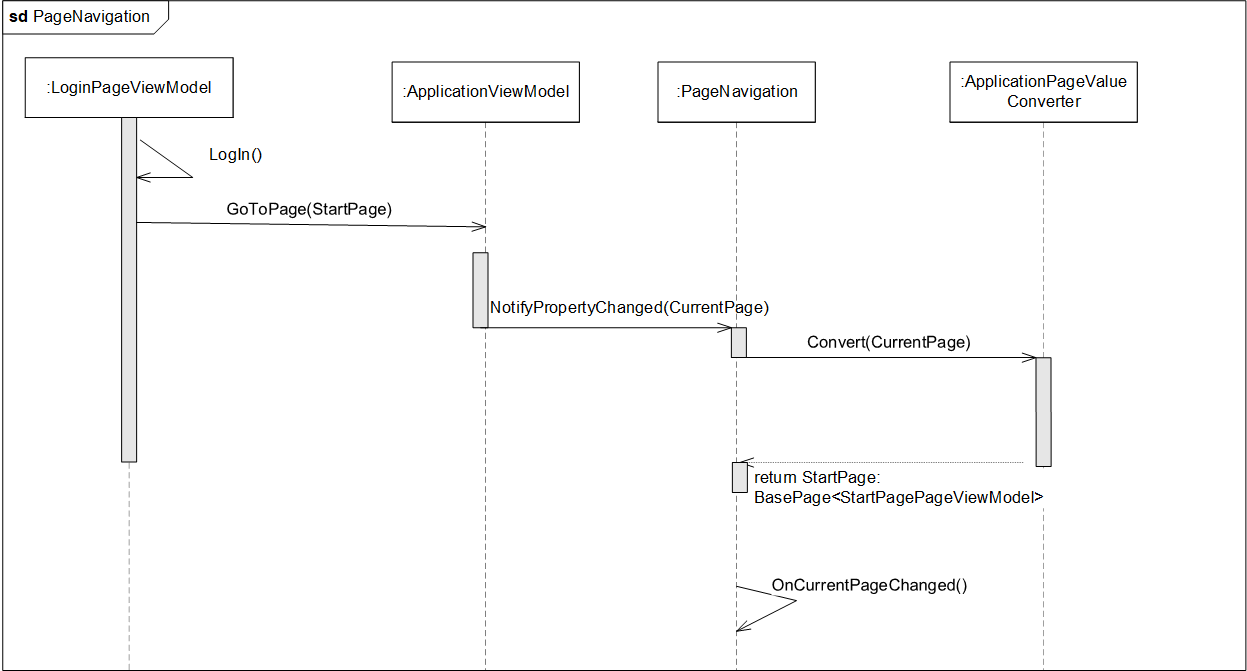
\includegraphics[width=\textwidth]{SoftwareDesign/MVVMDesigns/Graphics/PageNavigationSd.png}
    \caption{Her ses sekvensdiagrammet for PageNavigation, hvor Login skifter til StartPage Viewet}
    \label{fig:PageNavigation_SD}
\end{figure}

\subsubsection{Headerbar}
\textbf{Design af View - Headerbar}\\
Headerbaren er placeret i toppen af applikationen og kan findes på samtlige sider. Det er også gennem den, at man som bruger navigerer gennem applikationen ved brug af navigationsredskaber (knapper, osv). Det skal ikke være muligt at navigere fra Loginsiden, inden man er godkendt som bruger. Dette er den eneste undtagelse, hvor headerbaren ikke skal vises. Grænsefladen for Viewet tager udgangspunkt i figur \ref{fig:headerbar_wf}\\\\
\begin{figure}[H]
    \centering
    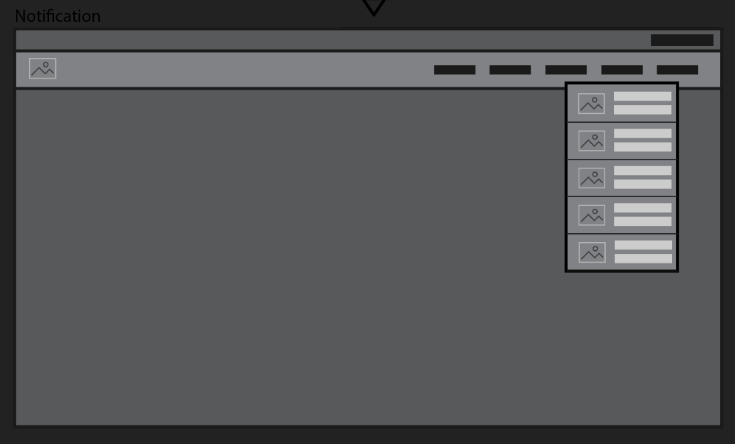
\includegraphics[width=\textwidth]{SoftwareDesign/MVVMDesigns/Graphics/HeaderBarWireFrame.png}
    \caption{Headerbar WireFrame}
    \label{fig:headerbar_wf}
\end{figure}
Der angives navigationsegenskaberne for Headerbaren i Wireframet, som blev introduceret i Arkitekturen (Se figur XX eller bilag \textbf{Wireframe}). \\\\
\textbf{Design af ViewModel - Headerbar}\\
Arkitekturen af Headerbaren er tæt tilknyttet til ApplicationPageViewModel. Hvert knap tilknyttes en kommando, som anvender ApplicationPage til at skifte side ved aktivering. Søgebaren er dog eventbaseret og aktiveres når brugeren indtaster en streng og trykker på søg (fx keyboard aktivering). Eventet sendes til SearchView og der navigeres til selvsamme side. \\\\
Et andet vigtig element i Headerbaren er notifikationsknappen, som ved aktivering, vises som en popup-menu i figur \ref{fig:headerbar_wf}. Menuens indhold er udliciteret til et separat View og ViewModel. 

\subsubsection{Beskeder \& Notifikationer}
\textbf{Design af View - Notification}\\
NotificationView udfoldes ved aktivering i Headerbaren. Brugeren præsenteres de 10 eller færre nyeste notifikationer. En notifikation indeholder kun de vigtigste informationer, da det ikke er muligt at vise alt indhold for en besked. Den visuelle repræsentation af vinduet kan ses i figur \ref{fig:wire_noti}. NotificationViewet kan ses som en beskedbeholder, hvor der kan opstå forskellige typer notifikation beskeder. Det er derfor essentielt, at det er let at tilføje nye typer beskeder/notifikationer. Der er to typer beskeder defineret for systemet: 
\begin{enumerate}
    \item Lejer anmoder om bil 
    \item Udlejer respons til anmodning
\end{enumerate}
\begin{figure}[H]
    \centering
    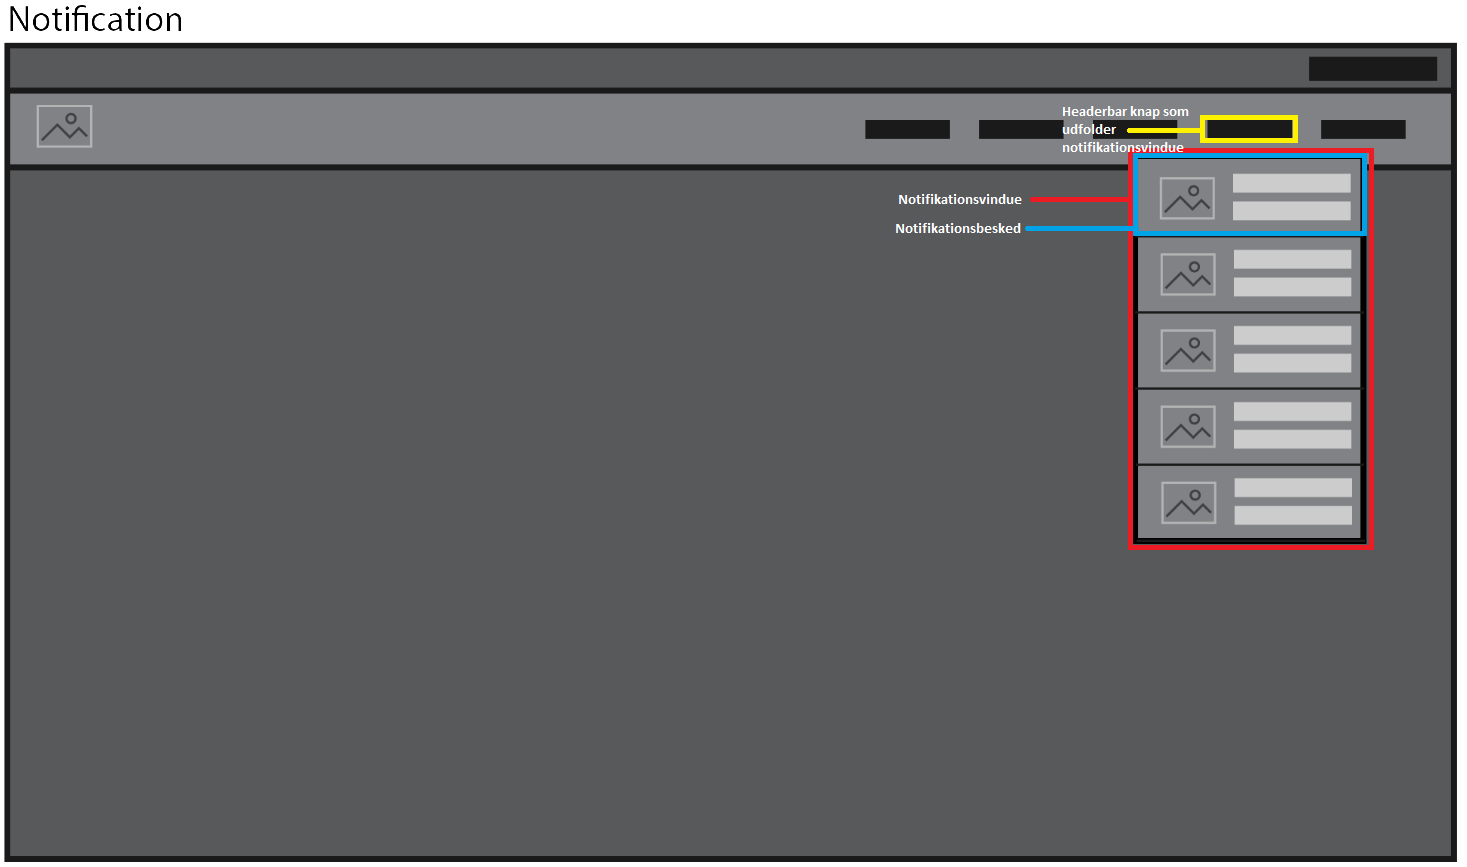
\includegraphics[width=\textwidth]{SoftwareDesign/MVVMDesigns/Graphics/noti_wirefame.png}
    \caption{WireFrame for Notifikations vinduet}
    \label{fig:wire_noti}
\end{figure}
Notifikationsvinduet laves som en UserControl, så den tilføjes til både Headerbaren og Messagevinduet. De individuelle views til beskederne, vil så kunne tilføjes.

\textbf{Design af ViewModel - Notification}\\
En bruger vil modtage notifikationer, når han interagerer med applikationen, specifikt når der enten lejes eller udlejes en bil. Hvert type besked vises forskelligt, og der skal derfor differentieres runtime mellem besked typerne. Hertil bruges en \textbf{value converter}, som konverterer indholdet af en besked til et 'WPF item', så det kan vises i Notifikationsvinduet (En notifikationsbesked er repræsenteret som en blok inde i vinduet, se figur \ref{fig:wire_noti}). Hvert besked har dets eget View og Model, og det angives typen af notifikationen i Modellen, herved kan konverteren differencier runtime mellem beskederne. Hvis systemet udvides og der tilføjes flere typer beskeder, kan de let tilføjes ved at oprette et nyt View og tilhørende Model. Figur \ref{fig:cd_noti} illustrerer strukturen af designet. 
\begin{figure}[H]
    \centering
    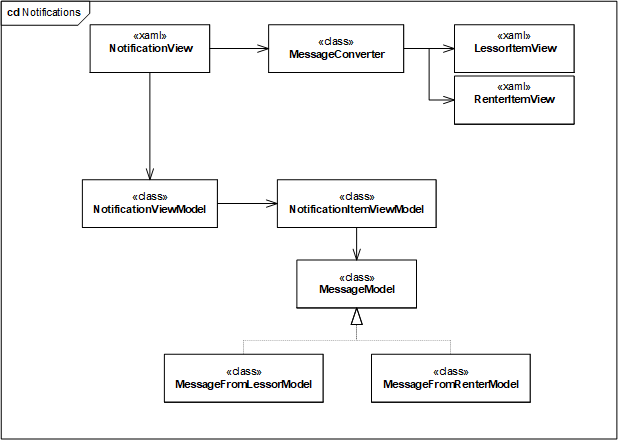
\includegraphics[width=\textwidth]{SoftwareDesign/MVVMDesigns/Graphics/cd_notification.png}
    \caption{Klassediagram for notifikationer}
    \label{fig:cd_noti}
\end{figure}


\textbf{Design af View - Message}\\
I forlængelse med Notifikationsvindeut, skal brugeren have adgang til alle modtaget beskeder. Hvert element i Notifikationsvinduet navigerer til Messagevinduet, hvor brugeren præsenteres til den fulde besked og alle tidligere beskeder (designet af vinduet ses i figur \ref{fig:wire_message}): 
\begin{enumerate}
    \item Den venstre side af vinduet viser alle brugerens beskeder 
    \item Den højre side viser indholdet af den besked, som brugeren har valgt
    \begin{itemize}
        \item Udlejer respons: Her vises beskeden fra udlejeren, samt om han har godkendt bilanmodningen
        \item Lejer anmodning: Her vises beskeden fra lejer - udlejeren kan godkende eller afvise anmodningen i Notifikationsvinduet. 
    \end{itemize}
\end{enumerate}
\begin{figure}[H]
    \centering
    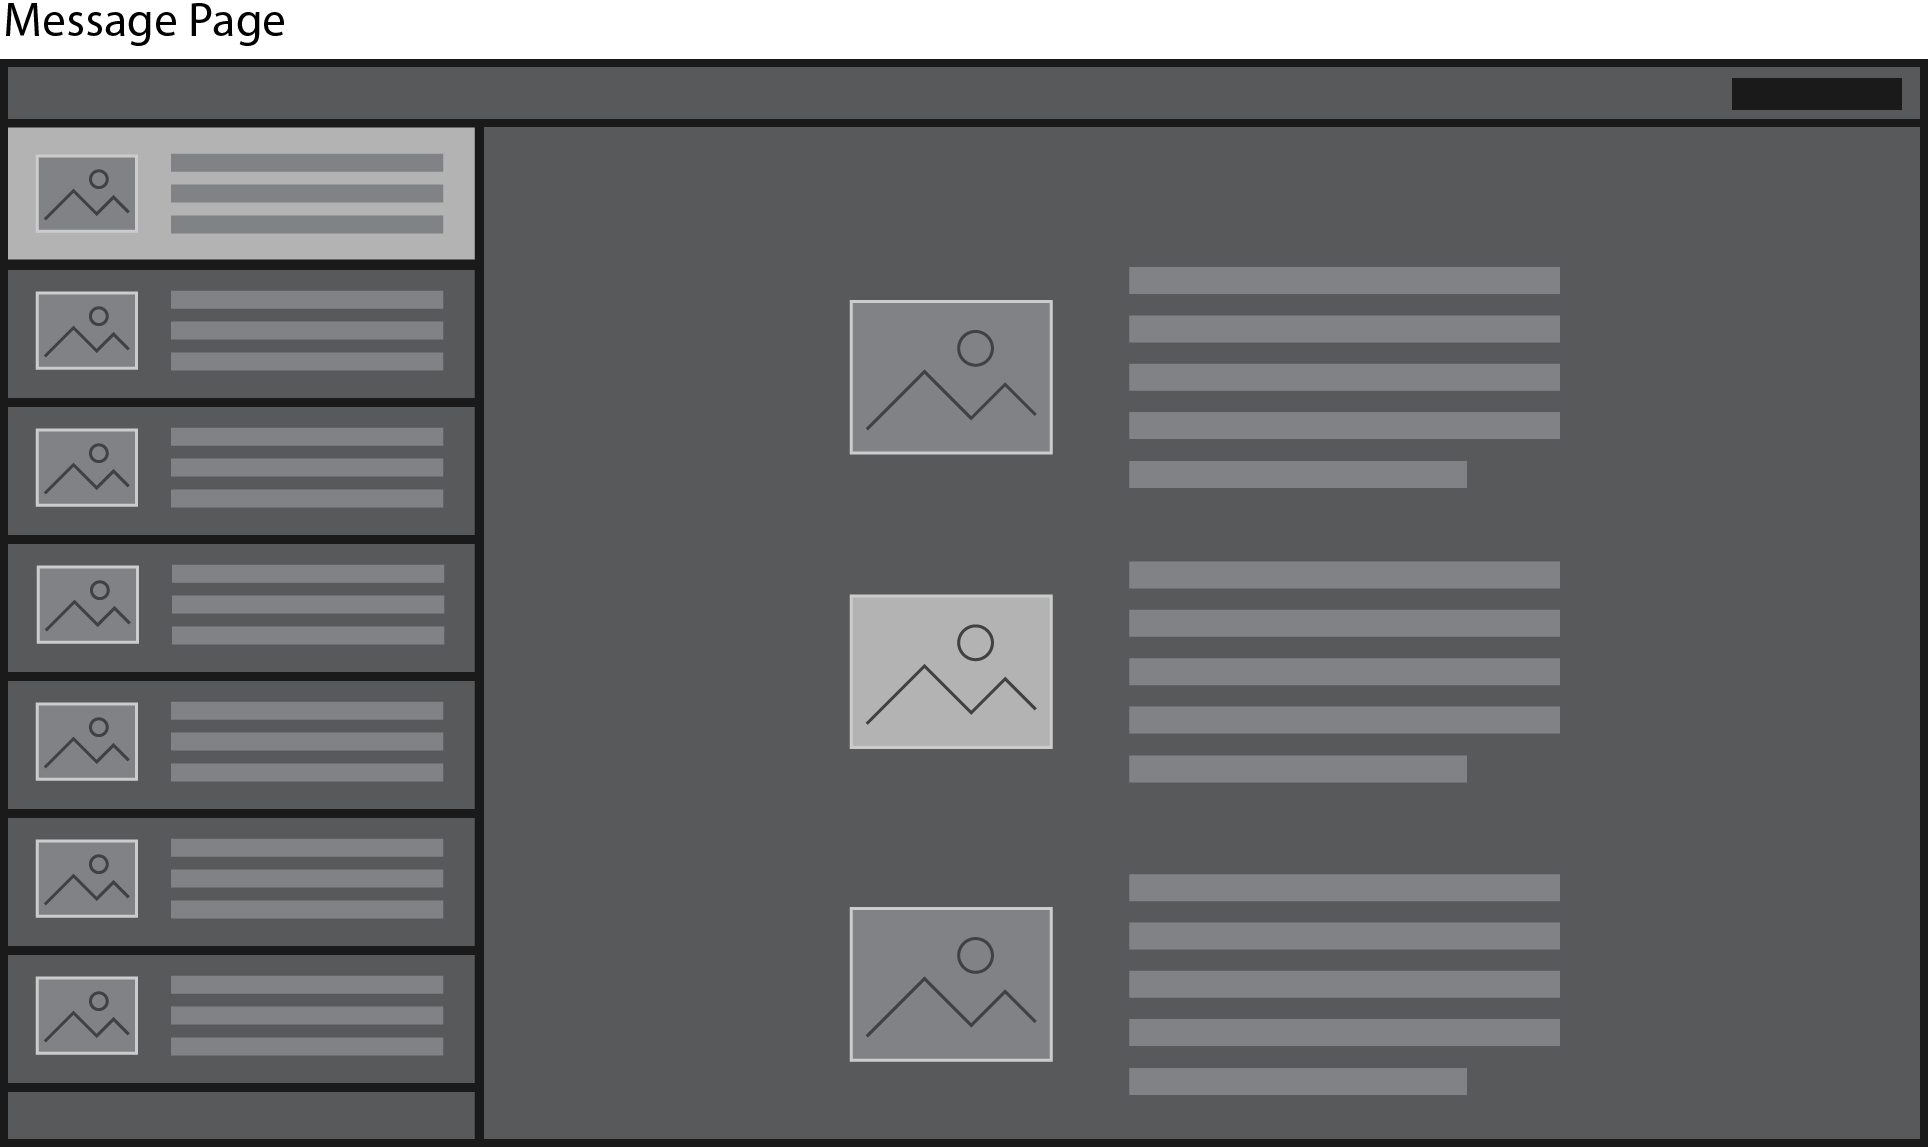
\includegraphics[width=\textwidth]{SoftwareDesign/MVVMDesigns/Graphics/MessageView.png}
    \caption{Frame for Message}
    \label{fig:wire_message}
\end{figure}

\textbf{Design af ViewModel - Message}\\
Brugerens beskeder vil være være et 1:1 forhold med Notifikationsvinduet, her vises de samme beskeder. Beskederne er dog ikke statisk, de loades igen, når brugeren skifter mellem Notifikationsvinduet og Messagevinduet. Idet brugeren vælger en besked/notifikation sendes et event til Messagevinduet, hvor eventet indeholder den specifikke besked. Alt indhold for beskeden vises på den højre side af viewet (se figur \ref{fig:wire_message}). 

\subsubsection{Login}
\textbf{Design af View - Login}\\
Loginsiden er det første brugeren ser, når applikationen eksekveres. Det overordnede wireframe viser navigationsegenskaberne for vinduet (se bilag \textbf{Wireframe}). Fra Loginsiden skal der ikke kunne navigeres til andre sider, da det ville komprimere programmet (der kan være data gemt fra tidligere brug af applikationen, fx en tidligere bruger, og det fjernes ved login). Brugeren kan vælge at registrere sig i systemet, hvis han/hun ikke har en konto. Figur \ref{fig:LoginWireframe} viser designet for vinduet. 
\begin{figure}[H]
    \centering
    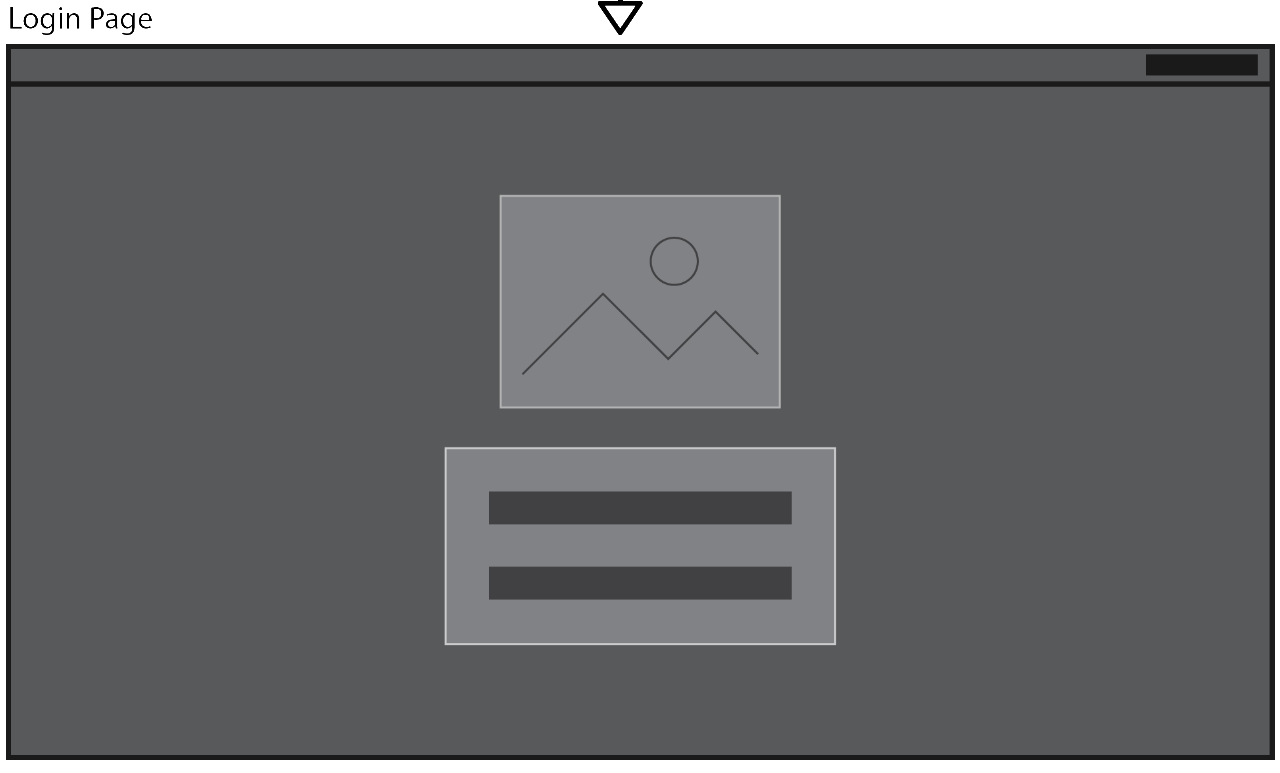
\includegraphics[width=\textwidth]{SoftwareDesign/MVVMDesigns/Graphics/LoginWireframe.png}
    \caption{Wireframe af login}
    \label{fig:LoginWireframe}
\end{figure}

\textbf{Design af ViewModel - Login}\\
Der er en del sikkerhedsforanstaltninger, som skal overholdes for login og konti (Tager udgangspunkt i kravene defineret i Security View, se afsnit XX i bilag \textbf{Arkitektur} og afsnit XX i bilag \textbf{Kravspecifikation}). Brugerens kodeord og email valideres. Koden er fortrolig information, som ikke skal vises i applikation. For at realiserer dette omdannes koden til typen securestring\cite{securestring}. Ved login navigeres videre til Startsiden, ellers kan der navigeres til Usersignup - dette sker via delagate commands. 


\subsubsection{Søgning}
\textbf{Design af View - Search}\\
Betegnelsen 'Search' dækker over den del af applikationen, som giver lejere mulighed for at finde og leje biler. Der er dedikeret en side i applikationen til søgefunktionaliteten, og designet af denne tager udgangspunkt i en WireFrame, som kan ses i figur \ref{fig:search_wireframe}. Det fremgår, at siden er delt i to. Som bruger skal man have mulighed for at se, hvilke biler, der er tilgængelige, dvs. de biler som tidligere er blevet registreret i systemet af en udlejer, og som nu kan lejes. Dette er vist til højre i figur \ref{fig:search_wireframe}, hvor der kan scrolles gennem udvalgte biler. Hver af de adskilte enheder repræsenterer én bil og indeholder således et billede, nogle relevante informationer vedrørende bilen og en knap, som giver brugeren mulighed for at leje den. \\\\Til venstre i figur \ref{fig:search_wireframe} er en række søgekriterier, som giver brugeren mulighed for at sortere i søgeresultaterne. Dermed behøver brugeren ikke at gennemgå samtlige biler, men kun de relevante biler, der opfylder de indtastede kriterier. Der foretages ikke gentagne søgninger i databasen. Det vurderes, at det er en bedre løsning at foretage en enkelt søgning, og vise brugeren et udsnit eller samtlige biler i databasen, som så efterfølgende kan blive filtreret. Selv om det betegnes 'Search' er det altså filtrering af søgeresultater, som er det essentielle, og dette er en del af præsentationslogikken. Med denne fremgangsmåde mindskes interaktionen med databasen, og derved er der mindre overhead og risiko for fejl.
\begin{figure}[H]
    \centering
    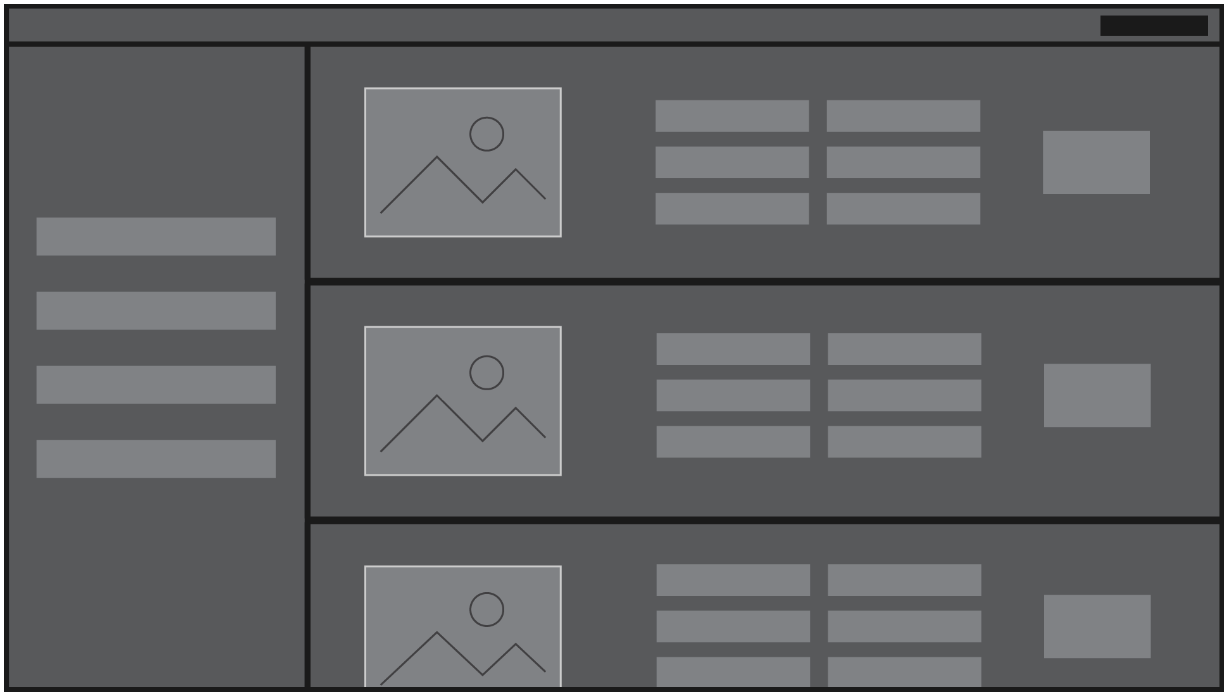
\includegraphics[width=\textwidth]{SoftwareDesign/MVVMDesigns/Graphics/SearchWireFrame.png}
    \caption{Search Page WireFrame}
    \label{fig:search_wireframe}
\end{figure}
For at kunne vise bilerne på en hensigtsmæssig måde er der lavet en UserControl med et billede af bilen og informationer om bilmærke- og model, lokation, pris, antal sæder og udlejers navn. Disse er bundet til properties i den ViewModel, som er tilknyttet, og som repræsenterer det enkelte søgeresultat (SearchResultItem ViewModel).

\textbf{Design af ViewModel - Search}\\
Der kan navigeres til Søgevinduet på to måder: Enten ved at trykke på 'Find Car' knappen eller søgebaren, som begge befinder sig i Headerbaren. Benyttelsen af søgebaren medfører at der navigeres til Search og foretages en filtrering efter lokation på baggrund af den indtastede streng. 

Den venstre side af vinduet består af flere filtreringskritirier og betingelser, som skal være opfyldt for brugeren. Systemet vil herefter query databasen efter biler, som opfylder prædikaterne. Hvis der ikke er udfyldt nogen kriterier vises alle bilerne, ellers skal alle prædikater være opfyldt for en given bil før den inkluderes i viewet - et prædikat kunne fx være billokation, antal sæder, udlejningsdato mv. Denne fremgangsmåde har fordelen, at hvert enkelt søgekriterie kan holdes simpelt og testes separat.

Der kan opstå tilfælde, hvor brugeren indtaster ugyldige værdier for kriterierne (fx hvis brugeren indtaster udlejningsdatoer, som ikke passer overens). Data valideres i forhold til brugerens input. Hvis der ikke er valgt en gyldig værdi, vil prædikatboksen vise en rød kant, og der vil blive udstedt passende fejlmeddelelse i tooltip. Det vil desuden ikke være muligt at foretage en søgning, hvis der er kriterier med ugyldig data. 


\subsubsection{Bilprofil}

\textbf{Design af View - Car Profile}
\\I dette afsnit beskrives designet for siden Bilprofil, og der tages udgangspunkt i en Wireframe, som kan ses i figur \ref{fig:CarProfileWireFrame}. Siden giver brugere mulighed for at sætte en bil til leje. Forudsætningen for, at man kan tilgå siden er, at man er registreret som udlejer, og først da bliver det muligt for brugeren at navigere til siden. Her har man mulighed for at indtaste oplysninger om bilen såsom bilmærke- og model samt bilens alder. Derudover kan der uploades et billede af bilen, og brugeren skal angive det tidsinterval, hvor bilen er tilgængelig for lejere.

\begin{figure}[H]
    \centering
    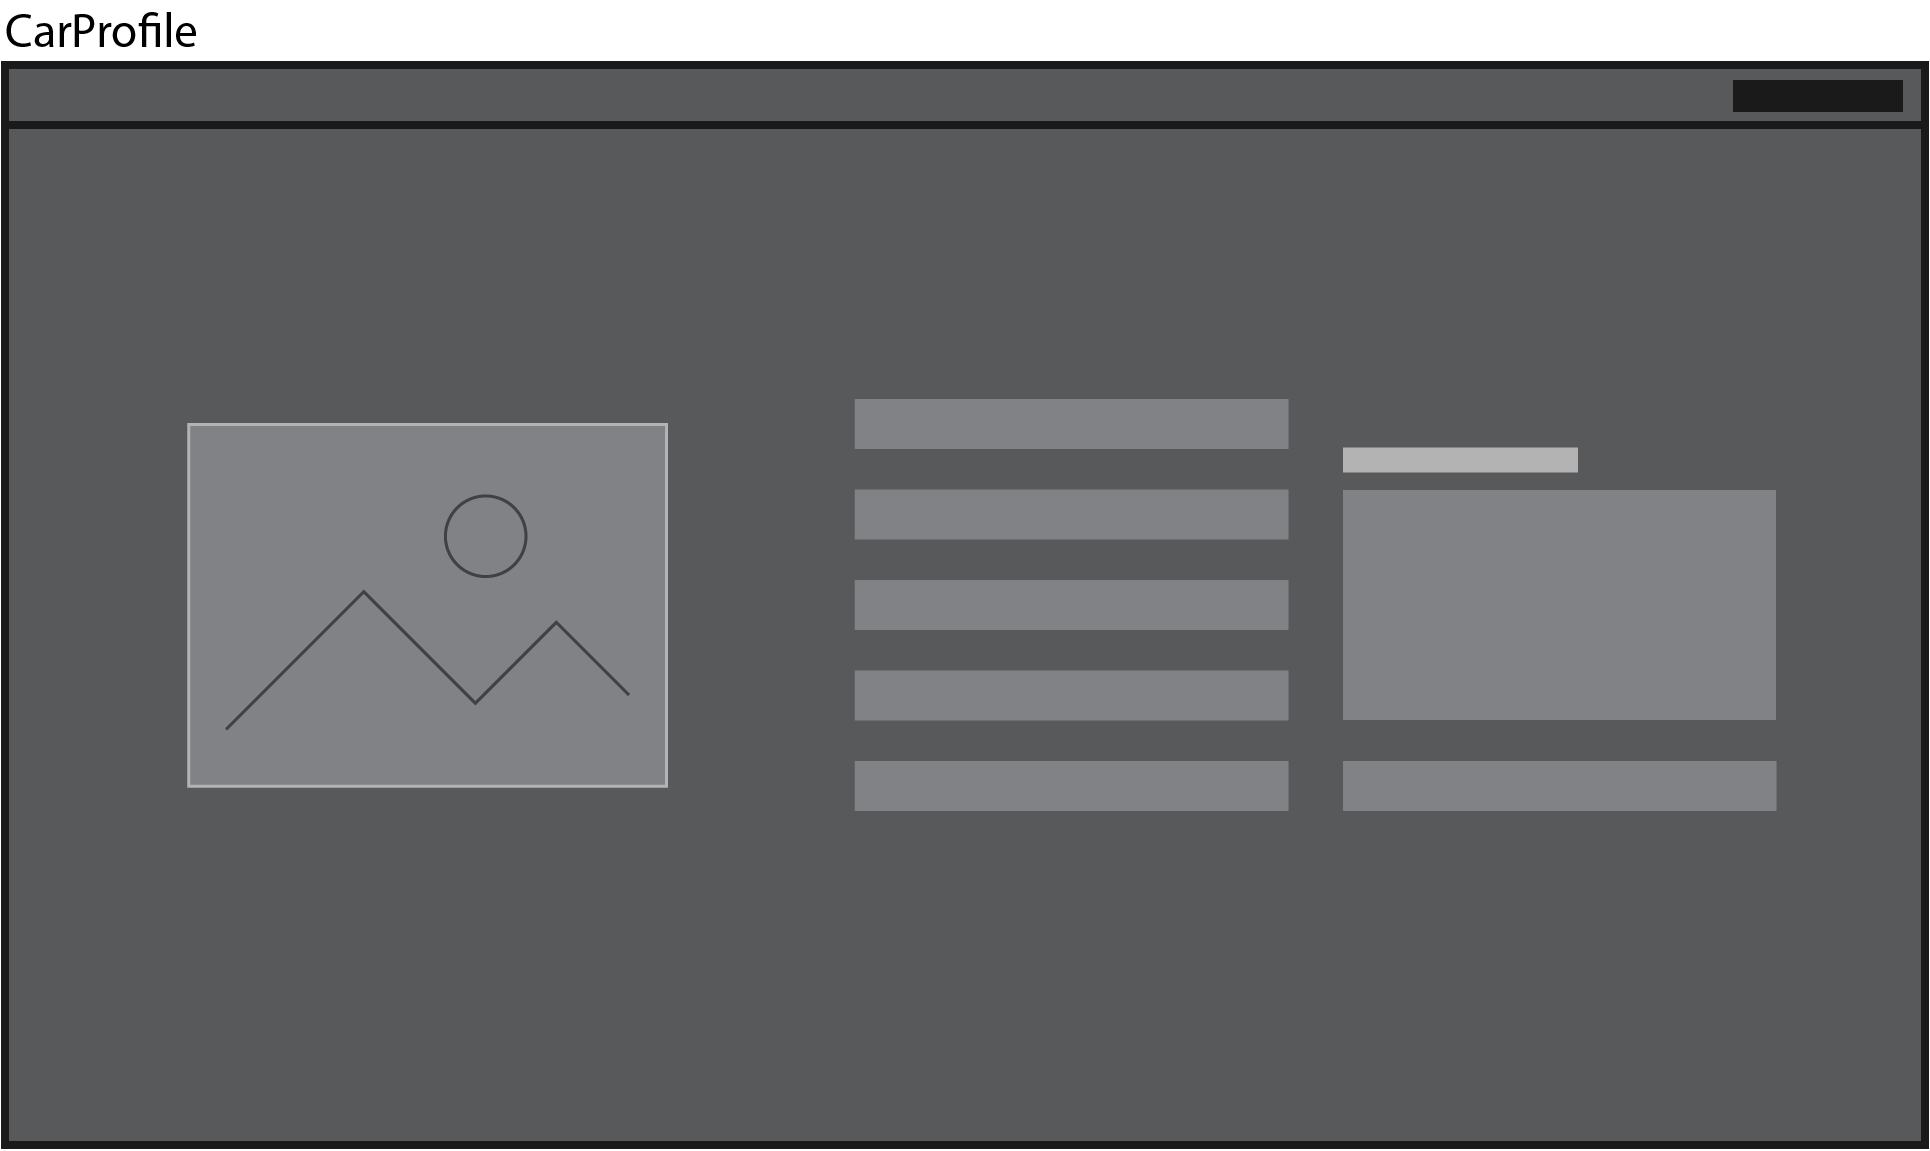
\includegraphics[width=\textwidth]{SoftwareDesign/MVVMDesigns/Graphics/CarProfileWireFrame.png}
    \caption{Car Profile WireFrame}
    \label{fig:CarProfileWireFrame}
\end{figure}

\textbf{Design af ViewModel - Car Profile}
\\Sidens funktionalitet varierer alt efter om udlejer registrerer bilen for første gang, eller blot opdaterer oplysninger for en allerede registreret bil. Som udgangspunkt er der mulighed for at gemme en ny bil med nye oplysninger. Hvis der allerede er registreret en bil giver siden kun mulighed for at redigere dennes oplysninger. Hvis udlejer vil uploade et billede af bilen åbnes en ny dialogboks, hvor man kan vælge et billede fra sin PC. Billedet lagres i applikationen, men konverteres til en streng før det lagres i databasen. 
\end{document}